\section{Entstehung des Gehirns}
%%%%%%%%%%%%%%%%%%%%%%%%%%%%%%%%%%%%%%%%%%%%%%%%%%%%%%%%%%%%%

\subsection{Neurulation}
\label{subsec:Neurulation} \index{Neurulation}
%%%%%%%%%%%%%%%%%%%%%%%%%%%%%%%%%%%%%%%%%%%%%%%%%%%%%%%

\begin{minipage}[b]{0.68\textwidth}
Der Embryo entwickelt drei Keimblätter: Endoderm, Mesoderm und Ektoderm. Aus diesen werden in späteren Entwicklungsschritten unterschiedliche Gewebe und Organe des adulten Individuums entstehen. Aus dem Mesoderm entstehen Skelett-, Muskel- und Bindegewebe, aus dem Endoderm Verdauungs-, Atem- und Urogenitaltrakt. Aus dem Ektoderm entstehen später die Haut und das Nervensystem \textsuperscript{\cite[Kap.~1]{crossman2014neuroanatomy}}. Die Entwicklung des Nervensystems beginnt mit der Neuralinduktion. Durch einen Anreiz des Mesoderms und der Chorda dorsalis bildet das darüber liegende Ektoderm das sogenannte Neuroektoderm aus. Das Neuroektoderm bildet dann die Neuralplatte (Abb.~\ref{fig:neurulation}). Im Laufe der Neurulation senkt sich diese in Richtung des Mesoderms ab und bildet so die Neuralrinne. Die angrenzenden Strukturen werden dadurch leicht erhöht und bilden die Neuralfalten. Durch weiteres Absinken und Abschnüren entsteht aus der Neuralrinne schließlich das Neuralrohr, aus den Neuralfalten die Neuralleisten. Aus der \textbf{Neuralleiste} werden im späteren Verlauf die Strukturen des peripheren Nervensystems entstehen. Aus dem \textbf{Neuralrohr} entwickelt sich das zentrale Nervensystem. Im Bereich des Kopfes bildet es das Gehirn aus, im hinteren Rumpfabschnitt das Rückenmark. Aus dem Hohlraum, den das Neuralrohr umschließt, entsteht das Ventrikelsystem\index{Ventrikelsystem} \textsuperscript{\cite[Kap.~1]{trepel2011neuroanatomie}}.
\end{minipage} \hspace{0.1cm}
\begin{minipage}[b]{0.3\textwidth}
\begin{figure}[H]
    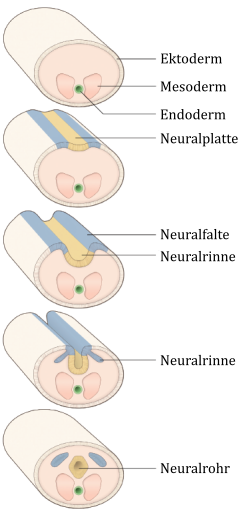
\includegraphics[width=\textwidth]{pictures/Bilder_Jule/Andere/Neurulation_crossm1.png}
    \caption[Neurulation]{\textbf{\\Neurulation.}\\
    Abbildung aus \textit{Neuroanatomy}, Crossman und Neary \textsuperscript{\cite[Kap.~1]{crossman2014neuroanatomy}}.}
    \label{fig:neurulation}
    \end{figure}    
\end{minipage} 

\subsection{Cephalisation}
\label{subsec:Cephalisation} \index{Cephalisation}
%%%%%%%%%%%%%%%%%%%%%%%%%%%%%%%%%%%%%%%%%%%%%%%%%%%%%%%
Zentrales und Peripheres Nervensystem der Wirbeltiere werden von unterschiedlichen ontogenetischen Strukturen gebildet. Das Periphere Nervensystem (PNS) wird aus Zellen der mesodermalen Neuralleiste gebildet. Im Gegensatz dazu wird das Zentrale Nervensystem (ZNS), das sowohl Gehirn als auch Rückenmark umfasst, von den Zellen des Neuralrohrs gebildet. Somit ist das ZNS ektodermalen Ursprungs. \\

\begin{figure}[H]
\centering
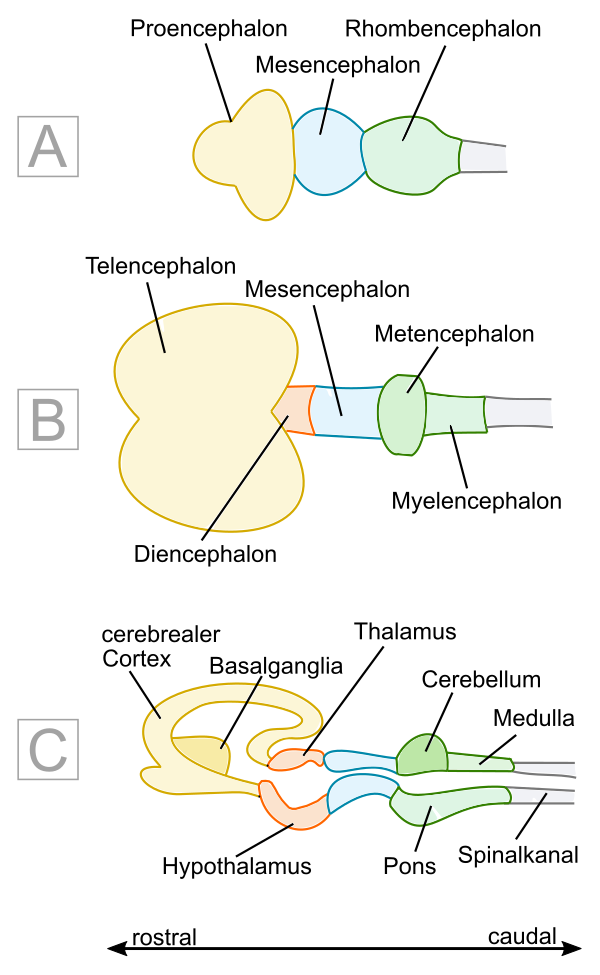
\includegraphics[width=0.5\textwidth]{pictures/Bilder_Jule/Andere/cephalisation.png}
\caption[Grundgliederung des Säugerhirns]{\textbf{Grundgliederung des Säugerhirns.} \textbf{A}:~primäre Hirnbläschen (3), \textbf{B}:~sekundäre Hirnbläschen (5), \textbf{C}:~Grundgliederung und Ventrikelsystem. \\
Abbildung nach \textit{Neurowissenschaften}, Bear et al. \textsuperscript{\cite[Kap.~7]{neurowissenschaften_baer}}.}
\label{fig:cephalisation}
\end{figure}

\noindent Im Laufe der Cephalisation bildet das frühe Neuralrohr rostral drei Schwellungen aus. Diese dehnen sich zunehmend aus und bilden die primären Hirnbläschen: Das Vorderhirn (Proencephalon)\index{Proencephalon}, Mittelhirn (Mesencephalon) und Rautenhirn (Rhombencephalon)\index{Rhombencephalon} (Abb.~\ref{fig:cephalisation}~A). Diese entwickeln sich im Laufe der Gehirnentwicklung zu den fünf sekundären Hirnbläschen: Das Proencephalon bildet zwei laterale Fortsätze aus, die cerebralen Ventrikel, die später die Hemisphären des cerebralen Cortex bilden werden. Zusammen mit dem rostralen Vorderhirn bilden sie das Endhirn (\textbf{Telencephalon})\index{Telencephalon}. Der caudale Teil des Vorderhirns bildet das Zwischenhirn (\textbf{Diencephalon})\index{Diencephalon}, aus dem Thalamus und Hypothalamus gebildet werden. Das Mittelhirn (\textbf{Mesencephalon})\index{Mesencephalon} formt vier Schwellungen, die zum inferioren und superioren Colliculus heranwachsen. Das Rautenhirn gliedert sich in Hinterhirn (\textbf{Metencephalon})\index{Metencephalon} und Nachhirn (\textbf{Myelencephalon})\index{Myelencephalon} auf, die später Pons und Cerebellum (Metencephalon), beziehungsweise die Medulla (Myelencephalon) bilden (Abb.~\ref{fig:cephalisation}~C). Zusammengefasst ist das Vertebratengehirn am Ende der Cephalisation in vier Teilbereiche gegliedert; Das Telencephalon, Diencephalon, Mesencephalon und das Rhombencephalon, das Met- und Myelencephalon zusammenfasst (Abb.~\ref{fig:cephalisation}~B) \textsuperscript{\cite[Kap.~10]{watson2010thebrain}}.

\subsection{Das Ventrikelsystem}
\label{subsec:} \index{Ventrikelsystem}
%%%%%%%%%%%%%%%%%%%%%%%%%%%%%%%%%%%%%%%%%%%%%%%%%%%%%%%

Jedes dieser Hirnventrikel umhüllt dabei einen mit Hirnwasser (\textit{Liquor cerebrospinalis}) gefüllten Hohlraum. Diese miteinander in Verbindung stehenden Ventrikel bilden das Ventrikelsystem (Abb.~\ref{fig:ventrikelsystem}), das auch als innerer Liquorraum  bezeichnet wird. Es besteht aus vier Ventrikeln: Zwei laterale Ventrikel, auch Seitenventrikel genannt, befinden sich im Telencephalon. Sie verlaufen entlang des Hippocampus, der ihre mediale Wand bildet. Der dritte Ventrikel befindet sich im Diencephalon. Im Gegensatz zu den lang gezogenen lateralen Ventrikeln befindet sich der dritte Ventrikel spaltförmig in der Midsagittalebene des Gehirns. Das Mesencephalon umgibt das Aquädukt (\textit{Aqueductus cerebri} oder \textit{Aqueductus mesencephali}). Es liegt unter der Vierhügelplatte und über dem Tegmentum. Der vierte und letzte Ventrikel ist im Rhombencephalon lokalisiert und erstreckt sich oberhalb des Hirnstamms und unterhalb des Cerebellums bis hin zum Rückenmark
\textsuperscript{\cite[Kap.~2]{watson2010thebrain}}.

\begin{figure}[H]
	\centering
	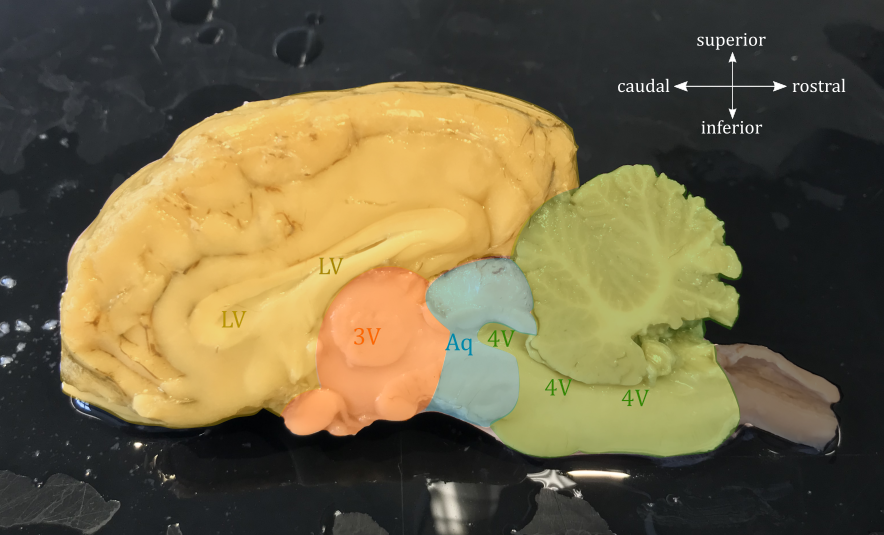
\includegraphics[width=0.8\textwidth]{pictures/Bilder_Jule/Andere/ventrikelsystem.png}
	\caption[Das Ventrikelsystem]{\textbf{Das Ventrikelsystem.} Das Ventrikelsystem im Midsagittalschnitt des Schafhirns. Das Telencephalon und der laterale Ventrikel (LV) sind gelb, Diencephalon und dritter Ventrikel (3V) orange, Mesencephalon und Aquädukt (Aq) blau und Rhombencephalon, sowie vierter Ventrikel (4V) grün gefärbt.}
	\label{fig:ventrikelsystem}
\end{figure}

\noindent Innerhalb der Ventrikel sind die \textbf{Plexus choroidei} \index{Choroid plexus} lokalisiert. Sie bestehen aus arterovenösen Gefäßästen, die von einem speziellen Epithel, dem Plexusepithel, überdeckt sind. Der Plexus choroideus produziert den Liquor\index{Liquor cerebrospinalis}, der das Gehirn umgibt. Dabei werden beim Menschen täglich, vor allem vom Plexus der lateralen Ventrikel, etwa 500~ml Liquor produziert. Diese klare Flüssigkeit, die nur wenige Zellen, hauptsächlich Leukozyten, und einen geringen Anteil an Eiweiß und Glucose enthält, dient als Druck- und Stoßdämpfer des Gehirns. Auch hält er das extrazelluläre Milieu konstant. Durch den Liquorfluss können zudem potentiell schädliche Metabolite entfernt werden \textsuperscript{\cite[Kap.~10]{trepel2011neuroanatomie}}. 